%%%%%%%%%%%%%%%%%%%%%%%%%%%%%%%%%%%%%%
%%%%%%%%%%%%%%%%%%%%%%%%%%%%%%%%%%%%%%
% Do not edit the TeX file your work
% will be overwritten.  Edit the RnW
% file instead.
%%%%%%%%%%%%%%%%%%%%%%%%%%%%%%%%%%%%%%
%%%%%%%%%%%%%%%%%%%%%%%%%%%%%%%%%%%%%%



We consider the problem of clustering time-course gene expression data. 
While thousands of genes might be simultaneously 
measured in a given genomics experiment, 
many genes may exhibit similar expression patterns.  
Clustering gene expressions
is one way to reduce the dimensionality of a complex data set 
and to facilitate scientific interpretations of intricate biological processes. 
Often, such dimensionality reduction is used for exploratory analysis and
is a first step before further downstream investigation.  
It is important, therefore, to ascertain the stability of the 
discovered clusters. 
 
We study a publicly available data set of mice gene expression
\citep{shoemaker:2015:ultrasensitive}.
Mice were infected with influenza virus,
and expression levels of a set of genes were assessed at 14 time points after infection.
Three measurements were taken at each time point (called biological replicates), 
for a total of $\ntimepoints = 42$ measurements per gene. 

\subsubsection*{The model}
Following \citet{Luan:2003:clustering} we apply cubic B-splines to 
smooth the time course expression data. 
Let $\x_\n\in\mathbb{R}^\ntimepoints$ be measurments of gene $\n$
at $\ntimepoints$ time points.
Let $\regmatrix$ be an $\ntimepoints \times \d$ regressor matrix.
In our case, the $ij$-th entry of $\regmatrix$
is the $j$-th B-spline basis vector evaluated at the
$i$-th time point. 
\figref{example_genes} shows measurements from an example gene and 
the B-spline basis. 

In this model, 
each component is characterized by a vector of regression coefficients
$\mu_\k$ and a variance $\tau^{-1}_\k$, so
$\beta_k = (\mu_\k, \tau_\k)$.
The distribution of the data arising from component $k$ is
\begin{align}\eqlabel{mice_model}
\p(\x_\n | \beta_\k, \b_\n) =
\normdist{\x_\n | \regmatrix\mu_\k + \b_\n,
\tau_\k^{-1}I_{\ntimepoints \times \ntimepoints}},
\end{align}
%
where $\b_\n$ is a gene-specific additive offset and $I$ is the identity matrix.
We include the additive offset because we
are interested in clustering gene expressions based on their patterns over time,
not their absolute level.
Notice that in this model, the shifts $\b_\n$ are local variables since they are unique to each gene $\n$. 

The mixture weights $\pi$ and cluster assignments $\z$ are drawn from the 
stick-breaking process described in \secref{model_bnp}. 

Our variational approximation factorizes similarly to \eqref{vb_mf}
except with an additional factor for the additive shift. 
In our variational approximation, we also make a simplification by letting
$\q(\beta_\k \vert \eta) = \delta (\beta_k \vert \eta)$, 
where $\delta(\cdot \vert \eta)$ denotes a point mass at a parameterized location. 
See \appref{app_mice} for further details concerning the model and
variational approximation. 


\begin{knitrout}
\definecolor{shadecolor}{rgb}{0.969, 0.969, 0.969}\color{fgcolor}\begin{figure}[!h]

{\centering 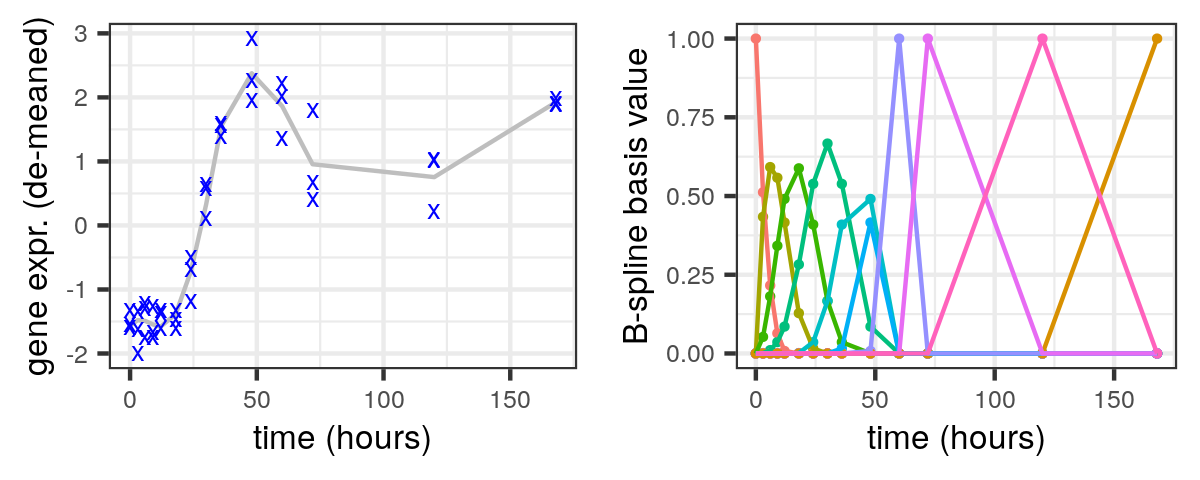
\includegraphics[width=0.980\linewidth,height=0.392\linewidth]{figure/example_genes-1} 

}

\caption[(Left) An example gene and its expression measured at 14 unique time points
    with three biological replicates at each time point.
     (Right) The cubic B-spline basis with 7 degrees of freedom, 
    along with three indicator functions for the last three time points, 
    $\timeindx = 72, 120, 168$]{(Left) An example gene and its expression measured at 14 unique time points
    with three biological replicates at each time point.
     (Right) The cubic B-spline basis with 7 degrees of freedom, 
    along with three indicator functions for the last three time points, 
    $\timeindx = 72, 120, 168$.}\label{fig:example_genes}
\end{figure}


\end{knitrout}
%

In this application, we expect to uncover finer structure
so we start with a larger $\alpha$ than the previous example 
and set $\alpha_0 = 6$. 
\figref{gene_initial_coclustering} displays the inferred co-clustering matrix
at this choice of $\alpha_0$. 
More precisely, let $\gcoclustering(\eta)\in\mathbb{R}^{\N\times\N}$ 
denote the co-clustering matrix, 
whose $(i,j)$-th entry is the
posterior probability that gene $i$ belongs to the same cluster
as gene $j$, given by 
\begin{align*}
[\gcoclustering(\eta)]_{ij}
&= \expect{\q(\z\vert\eta)}{\ind{\z_{i} = \z_{j}}} \\
&= \sum_{k=1}^{\kmax}\left(\expect{\q(\z_i\vert\eta)}{\z_{ik}}
\expect{\q(\z_j\vert\eta)}{\z_{jk}}\right).
\end{align*}

% $\gcoclustering(\eta)$, whose , given by 
% \begin{align*}
% \gcoclustering{ij}(\eta) 
% &= \expect{\q(\z\vert\eta)}{\ind{\z_{i} = \z_{j}}} \\
% &= \sum_{k=1}^{\kmax}\left(\expect{\q(\z_i\vert\eta)}{\z_{ik}}
% \expect{\q(\z_j\vert\eta)}{\z_{jk}}\right).
% \end{align*}

Below, we evaluate the sensitivity of the inferred co-clustering matrix to 
both parametric and functional perturbations to the stick distribution. 

\newcommand{\MiceSmoothers}{

\begin{knitrout}
\definecolor{shadecolor}{rgb}{0.969, 0.969, 0.969}\color{fgcolor}\begin{figure}[!h]

{\centering 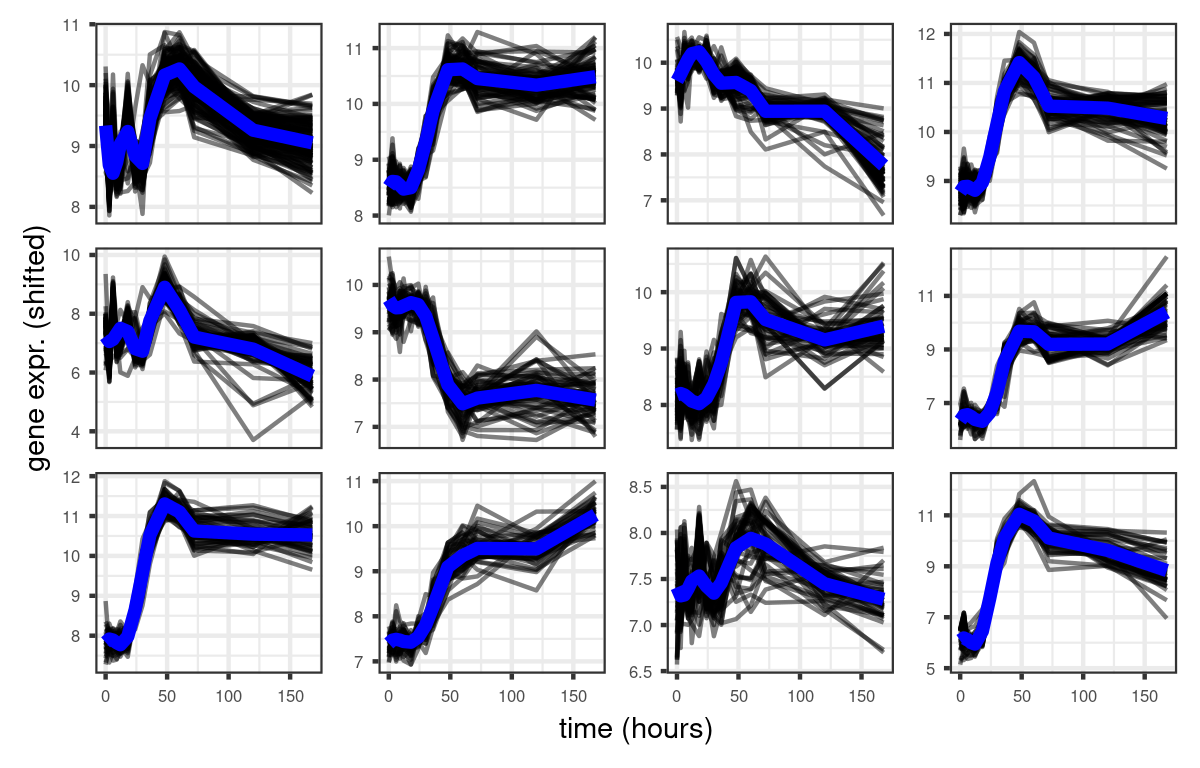
\includegraphics[width=0.980\linewidth,height=0.627\linewidth]{figure/gene_centroids-1} 

}

\caption[Inferred clusters in the mice gene expression dataset]{Inferred clusters in the mice gene expression dataset. 
    Shown are the twelve most occupied clusters. 
    In blue, the inferred cluster centroid. 
    In grey, gene expressions averaged over replicates and
    shifted by their inferred intercepts. }\label{fig:gene_centroids}
\end{figure}


\end{knitrout}
}



\begin{knitrout}
\definecolor{shadecolor}{rgb}{0.969, 0.969, 0.969}\color{fgcolor}\begin{figure}[!h]

{\centering 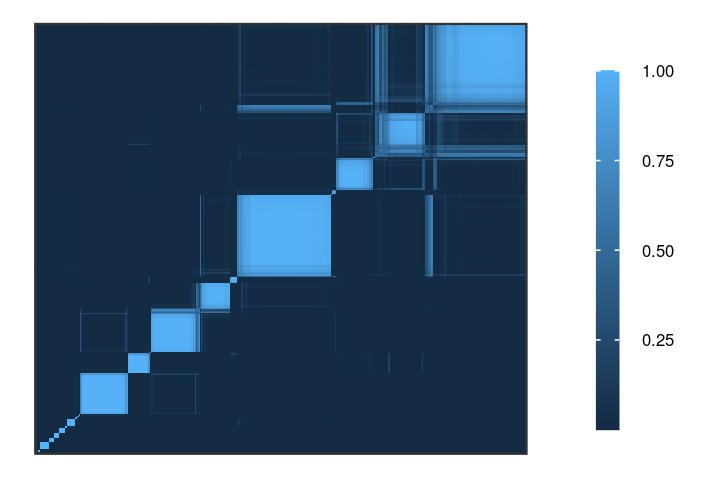
\includegraphics[width=0.588\linewidth,height=0.470\linewidth]{figure/gene_initial_coclustering-1} 

}

\caption[The inferred co-clustering matrix of gene expressions at $\alpha_0 = 6.$ ]{The inferred co-clustering matrix of gene expressions at $\alpha_0 = 6.$ }\label{fig:gene_initial_coclustering}
\end{figure}


\end{knitrout}


\subsubsection*{Sensitivity of co-clustering to $\alpha$}

We first evaluate the sensitivity of the co-clustering matrix $\gcoclustering$ 
to the choice of $\alpha$ in the
$\betadist{\nuk \vert 1, \alpha}$ stick-breaking distribution. 
Let $\gcoclustering^0 := \gcoclustering(\etaopt(\alpha_0))$ be the co-clustering matrix inferred at $\alpha_0$, 
and let $\Delta\gcoclustering(\eta) := 
\gcoclustering(\eta) - \gcoclustering^0$. 
We formed the linear approximation at $\alpha_0$ and computed
$\Delta\gcoclustering(\etalinglobal(\alpha))$, the 
the change in co-clustering under the linearized 
variational parameters, at $\alpha = 1$ and $\alpha = 11$. 
%(Note that the co-clustering matrix as a posterior quantity depends on only expectations of $\z$.
% We write $\gcoclustering(\etalinglobal)$ with the 
% understanding that the coclustering matrix is a function of global parameters $\etaglob$ only through its corresponding local parameters $\eta_\z$).

For either $\alpha$, the change in the posterior co-clustering 
matrix is minuscule (\figref{gene_alpha_coclustering}):
the largest entry of either matrix $\Delta\gcoclustering(\etalinglobal(1))$ 
or $\Delta\gcoclustering(\etalinglobal(11))$ is of order $10^{-2}$.
Refitting the approximate posterior at $\alpha = 1$ and $\alpha = 11$ 
and computing $\Delta\gcoclustering(\etaopt(\alpha))$
confirms the insensitivity predicted by the 
linearized variational global parameters.  
Beyond capturing insensitivity, the linearized parameters 
were also able to
approximate the sign and size of the changes in the individual entries of the coclustering matrix (these changes albeit small).  


\begin{knitrout}
\definecolor{shadecolor}{rgb}{0.969, 0.969, 0.969}\color{fgcolor}\begin{figure}[!h]

{\centering 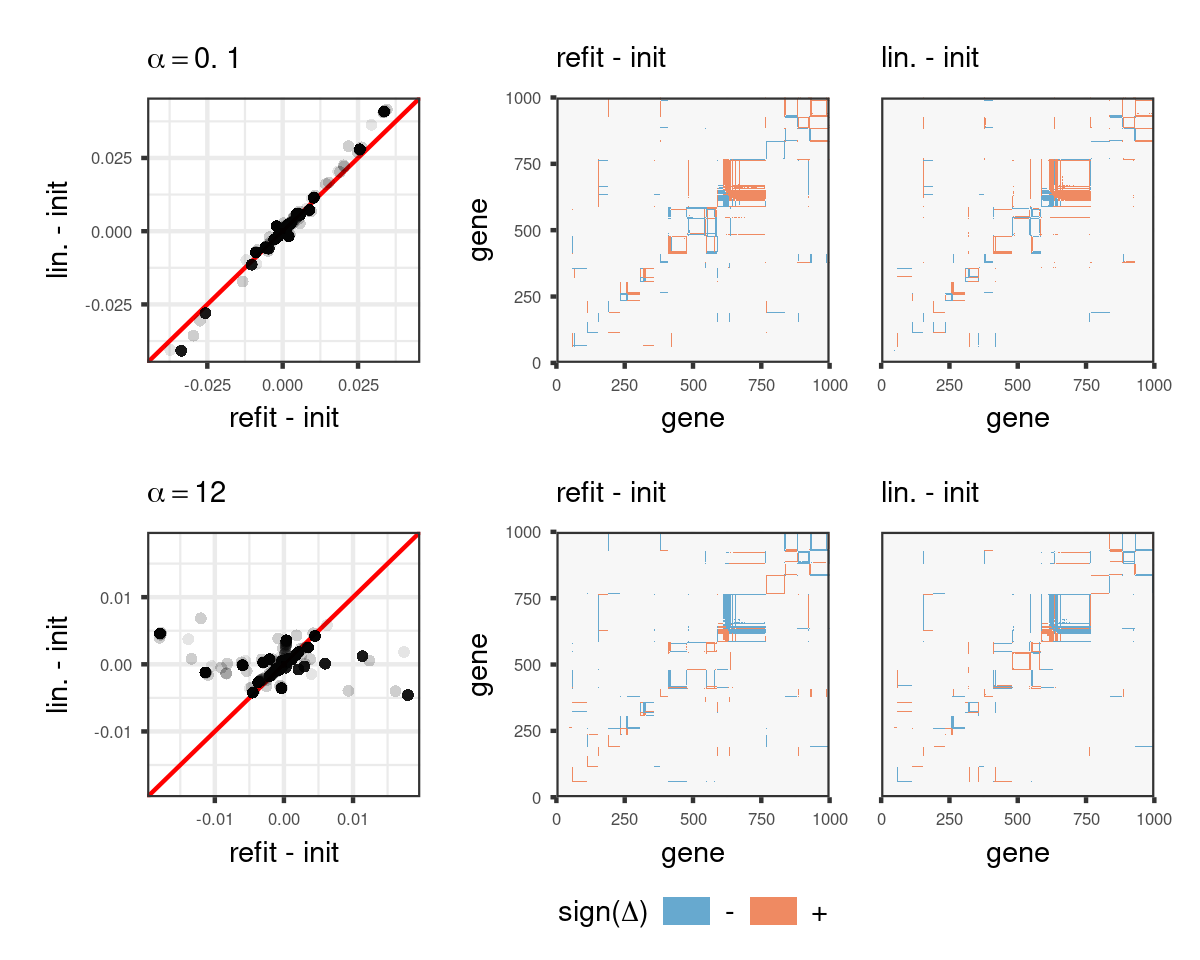
\includegraphics[width=0.980\linewidth,height=0.784\linewidth]{figure/gene_alpha_coclustering-1} 

}

\caption[Differences in the 
     co-clustering matrix at $\alpha = 1$ (top row)
     and $\alpha = 11$ (bottom row),
     relative to the co-clustering matrix at $\alpha_0 = 6$.
     (Left) a scatter plot of differences under the linear approximation 
     against differences after refitting, where
     each point represents an entry of the co-coclustering matrix.
     Note the scales of the axes]{Differences in the 
     co-clustering matrix at $\alpha = 1$ (top row)
     and $\alpha = 11$ (bottom row),
     relative to the co-clustering matrix at $\alpha_0 = 6$.
     (Left) a scatter plot of differences under the linear approximation 
     against differences after refitting, where
     each point represents an entry of the co-coclustering matrix.
     Note the scales of the axes: 
     the largest change in an entry of the co-clustering matrix is 
     $\approx 0.03$.  
     (Middle) sign changes in the co-clustering matrix observed after refitting. 
     (Right) the changes under the linearly approximated variational
     parameters. 
     For visualization, changes with absolute value $< 1e-5$ are not colored. }\label{fig:gene_alpha_coclustering}
\end{figure}


\end{knitrout}

\subsubsection*{Sensitivity of co-clustering to a functional perturbation}

Insensitivity to $\alpha$ does not necessarily rule out insensitivity to other prior perturbations, however. 
As demonstrated in \secref{results_iris},
the influence function can provide guidance on which functional perturbations may result in greater sensitivity for a chosen posterior quantity. 
However, the co-clustering matrix as a posterior quantity is 
$\ngenes^2$-dimensional and 
thus does not lend itself to an easily interpretable influence function. 
We therefore summarize the co-clustering matrix into a scalar quantity: 
we use the sum of the eigenvalues of the symmetrically normalized graph Laplacian. 
This quantity has close connection with 
the number of distinct components in a graph~\citep{luxburg:2007:spectralcluster}. 
Let this posterior quantity be denoted $\laplacianevsum$, given by 
\begin{align*}
  \laplacianevsum(\eta) = 
  \text{Tr}\left(
  I - D(\eta)^{-1/2} \gcoclustering(\eta) D(\eta)^{-1/2}
  \right),
\end{align*}
where $D(\eta)^{-1/2}$ is the diagonal matrix with entries $d_i = \sum_{j=1}^{\ngenes}[\gcoclustering(\eta)]_{ij}$. 
(And recall that the trace of a matrix is equivalent to the sum of its eigenvalues).

Because $\laplacianevsum(\eta)$ is a scalar quantity, we can plot its influence function. 
We choose a functional perturbation $\phi_{\textrm{ev}}$ that has a large, positive inner-product with the influence function.
In this case, we construct $\phi_{\textrm{ev}}$
using two Gaussian bumps aligned with
the two largest modes of the prior-weighted influence function
(\figref{gene_fpert_coclustering} top left). 
We anticipate $\phi_{\textrm{ev}}$
to have a large effect on $\laplacianevsum$. 
With $\laplacianevsum$ a proxy for our actual posterior quantity of interest, 
the full co-clustering matrix, we then expect that the co-clustering matrix 
will also experience large changes. 





Our intuition is confirmed in \figref{gene_fpert_coclustering}. 
After perturbing by $\phi_{\textrm{ev}}$, 
the largest changes in the co-clustering matrix are of now of order $10^{-1}$, 
compared with changes on the order of $10^{-2}$ after the $\alpha$ perturbations. 
The linearized variational parameters are again able to capture the qualitative changes in the co-clustering matrix after refitting at the perturbed prior. 


\begin{knitrout}
\definecolor{shadecolor}{rgb}{0.969, 0.969, 0.969}\color{fgcolor}\begin{figure}[!h]

{\centering 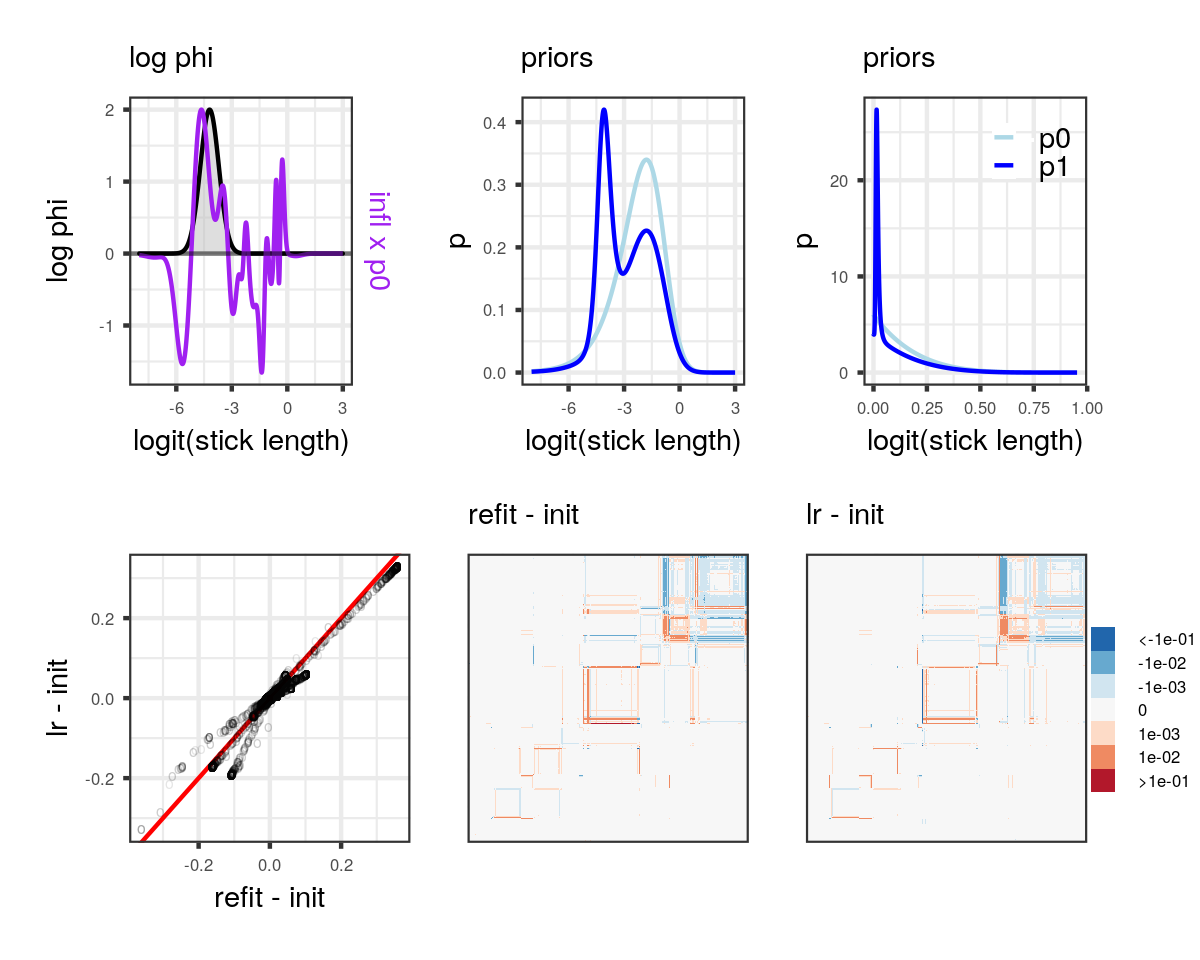
\includegraphics[width=0.980\linewidth,height=0.823\linewidth]{figure/gene_fpert_coclustering-1} 

}

\caption[Effect on the co-clustering matrix after a multiplicative functional
     perturbation.
     (Top left) the perturbation $\phi$ in grey, 
     and the influence function in purple]{Effect on the co-clustering matrix after a multiplicative functional
     perturbation.
     (Top left) the perturbation $\phi$ in grey, 
     and the influence function in purple. 
     (Top right) the effect of this perturbation on the prior density. 
     (Bottom) the effect of this perturbation on 
    the coclustering matrix.
    Note the scale of the scatterplot axes compared with
    the scatterplots in \figref{gene_alpha_coclustering}. }\label{fig:gene_fpert_coclustering}
\end{figure}


\end{knitrout}

The influence function is able to explain why the co-clustering matrix is 
insensitive to $\alpha$.
The functional perturbation
that corresponds to a change in $\alpha$ is
\begin{align*}
\phi_\alpha(\nu_\k) :=
\log\betadist{\nu_\k\vert 1, \alpha} -
\log\betadist{\nu_\k\vert 1, \alpha_0}.
\end{align*}
The function $\phi_\alpha(\nu_\k)$ is large when the influence function is small and vice-versa (\figref{alpha_pert_logphi}),
resulting in a small inner-product between the influence function
and $\phi_\alpha$. 
Thus, the linear approximation will predict small changes, and 
the refitted results confirms the predictions.  


\begin{knitrout}
\definecolor{shadecolor}{rgb}{0.969, 0.969, 0.969}\color{fgcolor}\begin{figure}[!h]

{\centering 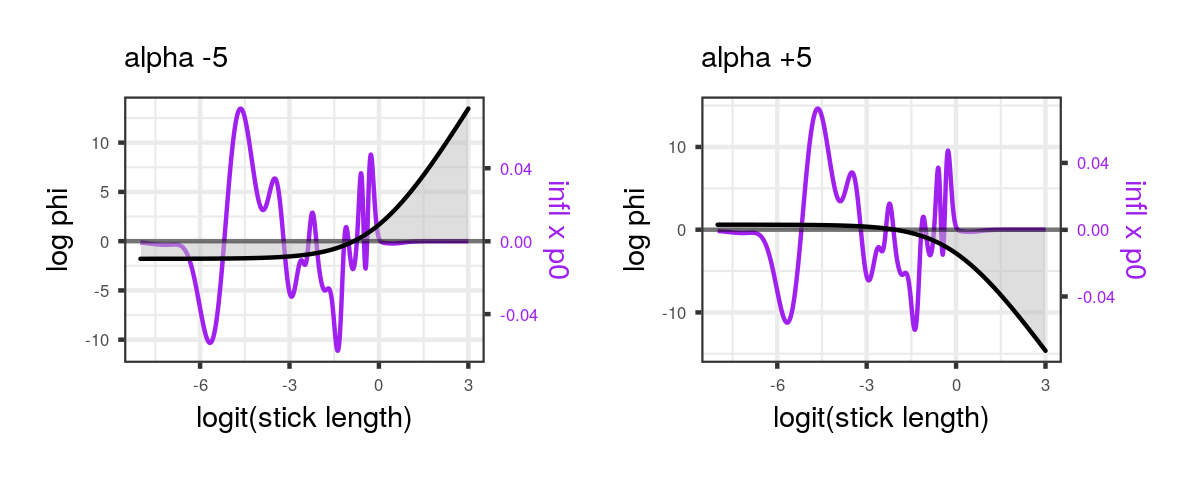
\includegraphics[width=0.882\linewidth,height=0.423\linewidth]{figure/alpha_pert_logphi-1} 

}

\caption[The multiplicative perturbations $\phi_\alpha(\cdot)$ that 
    corresponds to decreasing (left) or increasing (right) 
    the $\alpha$ parameter by five]{The multiplicative perturbations $\phi_\alpha(\cdot)$ that 
    corresponds to decreasing (left) or increasing (right) 
    the $\alpha$ parameter by five. }\label{fig:alpha_pert_logphi}
\end{figure}


\end{knitrout}

However, even with the selected functional perturbation,
the size of the differences in the co-clustering matrix remains modest. 
It is unlikely that any conclusions derived from the co-clustering matrix would have changed after the functional perturbation. 
The co-clustering matrix appears insensitive to perturbations in the stick-breaking distribution. 

Finally, the computational cost of linearizing the variational parameters is favorable compared with refitting (\tabref{mice_timing}). 
Forming the linear approximation, which requires a Hessian inversion, 
took 3-4 seconds; subsequent evaluations of $\etalinglobal$ take milliseconds. Conversely, refitting the model after a prior perturbation can take up to 20 seconds. 

\begin{table}[tb]
\centering
\caption{Compute time of results on the mice data set. }
\tablabel{mice_timing}
\begin{tabular}{|r|r|}
    \hline 
    & time (seconds) \\ 
    \hline 
    Initial fit & 25 \\
    \hline 
    Hessian solve for $\alpha$ sensitivity & 
        3.3\\
    Linear approx. $\etalinglobal(\alpha)$ for $\alpha = 1$ & 
        0.0015\\
    Linear approx. $\etalinglobal(\alpha)$ for $\alpha = 11$ & 
        0.00095\\
    Refit $\etaopt(\alpha)$ for $\alpha = 1$ & 
        14\\
    Refit $\etaopt(\alpha)$ for $\alpha = 11$ & 
        50\\
    \hline
    The influence function & 3.4\\ 
    Hessian solve for $\phi$ perturbation &
        2.8\\
    Linear approx. $\etalin(\t)$ at $\t = 1$ &
        0.00094\\
    Refit $\etaopt(\t)$ at $\t = 1$ &
        26\\
    \hline
\end{tabular}
\end{table}
